\section{Risultati}\label{sec:risultati}
  I risultati numerici delle misure sono riportati in tabella \ref{tab:risultati}.
  Abbiamo svolto le misure con $V_R = 2.0V$ e $R = 40k\Omega$ e usando
  un onda sinusoidale di frequenza $1kHz$.
  Le incertezze riportate sono calcolate nel modo standard
  (somma in quadratura di incertezza sistematica e incertezza casuale).
  La misura del tempo di salita è stata effettuata tra il 10\% e il 90\%
  dell'ampiezza totale dell'onda.
  La resistenza critica riportata corrisponde al valore di $R$ per cui si
  apprezza un cambiamento della curvatura della tosatura (in particolare,
  abbiamo osservato un cambiamento di $\frac 1 3$ di tacca dell'oscilloscopio).
  La figura \ref{fig:dati-raccolti} mostra il comportamento del
  circuito, rispetto alla variazione di $V_R$.
  \begin{figure}[H]
   \centering
      \begin{subfigure}{0.3\textwidth}
        \centering
        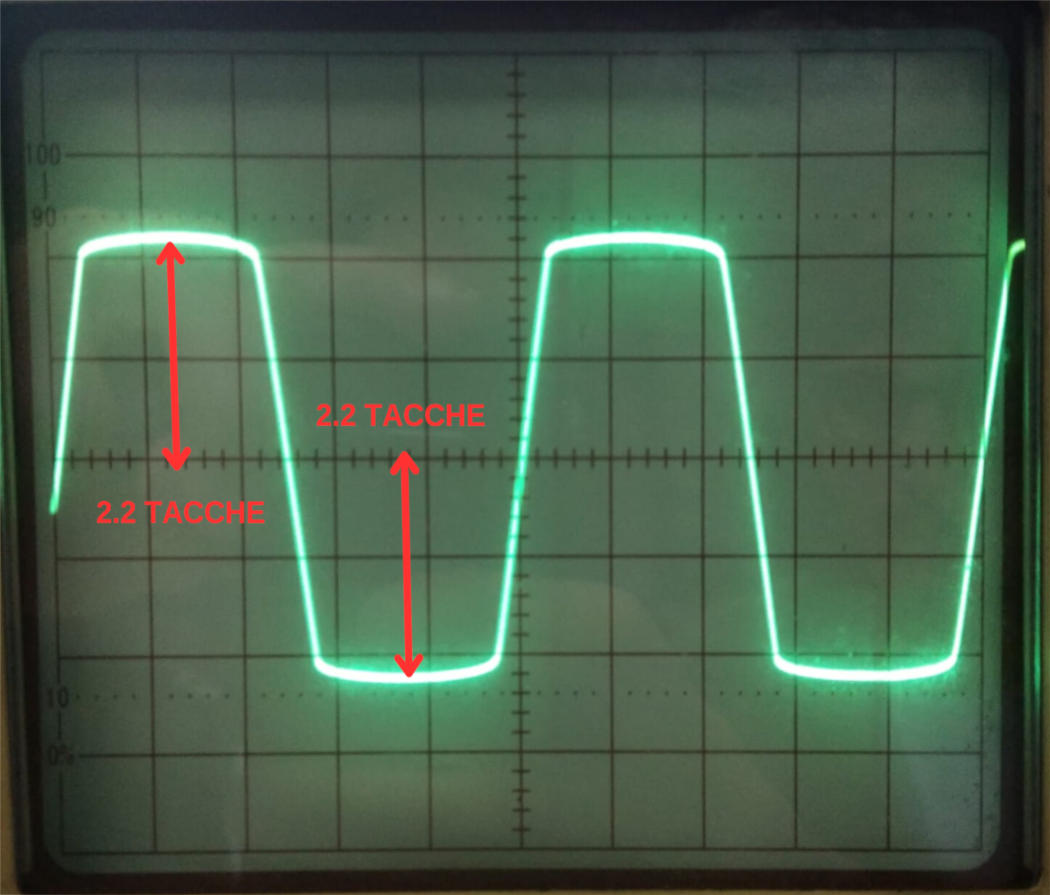
\includegraphics[width=\textwidth]{../assets/Resistenze_Uguali.png}
        \caption{\emph{Onda quadra generata con resistenze uguali.}}
        \label{fig : resistenze uguali}
      \end{subfigure}
      \hfill
      \begin{subfigure}{0.3\textwidth}
        \centering
        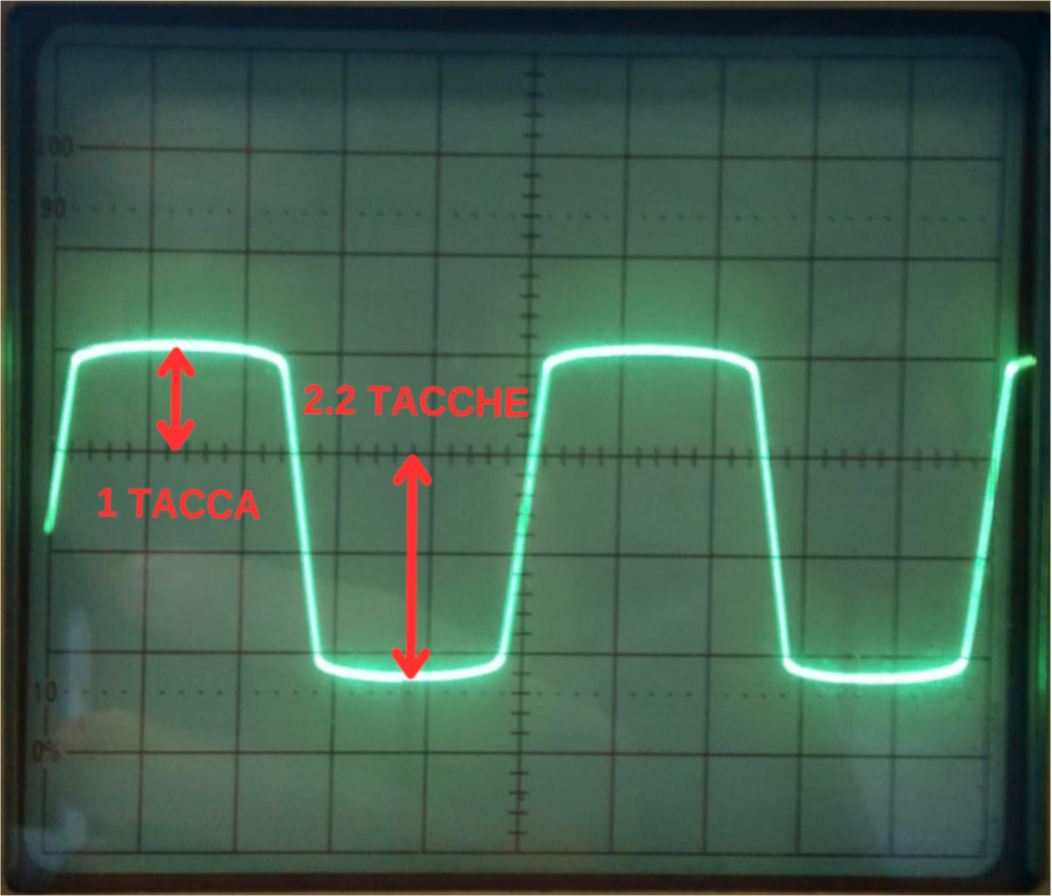
\includegraphics[width=\textwidth]{../assets/Resistenze_Diverse.png}
        \caption{\emph{Onda quadra generata variando una sola delle due resistenze.}}
        \label{fig : resistenze diverse 1}
      \end{subfigure}
      \hfill
      \begin{subfigure}{0.3\textwidth}
        \centering
        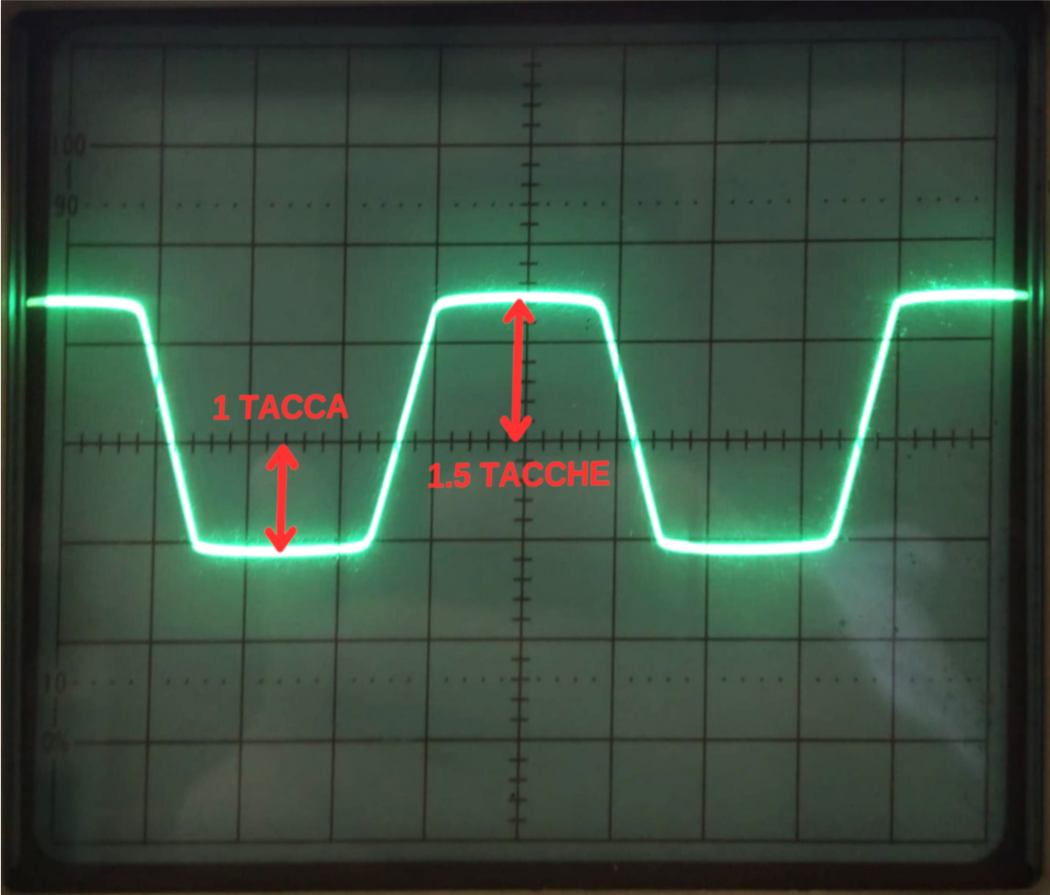
\includegraphics[width=\textwidth]{../assets/Resistenze_Diverse2.png}
        \caption{\emph{Onda quadra generata variando entrambe le resistenze.}}
        \label{fig : resistenze diverse 2}
      \end{subfigure}
      \caption{\emph{Onde quadre generate dal circuito variando i valori delle due resistenze.}}
    \label{fig:dati-raccolti}
  \end{figure}
\begin{table}[H]
  \centering
  \begin{tabular}[t]{c | p{3cm}  p{3cm}  p{3cm}  p{3cm}}
    \hline
    & Semiampiezza ($V$) & Semiampiezza tosata ($V$) & Tempo di Salita ($\mu s$) & Resistenza critica ($k \Omega$) \\
    \hline
    Silicio & $5.8 \pm 0.2$ & $2.55 \pm 0.09$ & $52.0 \pm 1.9$ & $35.90 \pm 0.16$ \\
    Germanio & $5.7 \pm 0.2$ & $2.10 \pm 0.08$ & $48.0 \pm 1.8$ & $34.33 \pm 0.16$ \\
    \hline
  \end{tabular}
  \caption{\emph{Caratteristiche misurate delle onde}}
  \label{tab : risultati}
\end{table}
